

\section{Discussion}

\subsection{Modal Decomposition Identifies Weathering Reaction}

The first step towards quantifying the extent to which chemical weathing reactions have gone to completion is to discern what reaction is taking place. In principle this is as simple as knowing what minerals are dissolving and which are precipitating. Modal decomposition methods consider several minerals that could be dissolving and/or precipitating, and their stoichiometry (Garrels and Mackenzie, 1967; Drever, 1997).


\begin{center}
\[
  \begin{bordermatrix}
{ & Biot & Plag & Calc & Smec & Kaol & KSpar \cr
Si  & a_{11}  & a_{12}  & a_{13}  & a_{14}  & a_{15}  & a_{16}  \cr
Al  & a_{21}  & a_{22}  & a_{23}  & a_{24}  & a_{25}  & a_{26}  \cr
Mg  & a_{31}  & a_{32}  & a_{33}  & a_{34}  & a_{35}  & a_{36}  \cr
Ca  & a_{41}  & a_{42}  & a_{43}  & a_{44}  & a_{45}  & a_{46}  \cr
Na  & a_{51}  & a_{52}  & a_{53}  & a_{54}  & a_{55}  & a_{56}  \cr
K   & a_{61}  & a_{62}  & a_{63}  & a_{64}  & a_{65}  & a_{66}  \cr}
  \end{bordermatrix}
  \cdot
  \begin{bordermatrix}
{ &  \cr
  & x_{Biot} \cr
  & x_{Plag} \cr
  & x_{Calc} \cr
  & x_{Smec} \cr
  & x_{Kaol} \cr
  & x_{KSpar} \cr}
  \end{bordermatrix}
  =
  \begin{bordermatrix}
{ & Spring (\mu mol/l) \cr
  & b_1 \cr
  & b_2 \cr
  & b_3 \cr
  & b_4 \cr
  & b_5 \cr
  & b_6 \cr}
  \end{bordermatrix}
\]
\end{center}
\bsk

Matrix algebra facilitates the calculations of the mineral proportions in the water. Given known matrices \( A \) and \( B \):

\begin{equation}
AX = B
\end{equation}
\begin{equation}
X = A^{-1}B
\end{equation}\\

This way, volumetric proportions of the minerals in the water can be calculated. Modal decompostion for spring waters was performed according to stoichiometric proportions from Bickle et al. (2015). For ease of visualisation, Figure 6 shows the positive, dissolved minerals on the LHS, and the negative, precipitated minerals on the RHS. \textcolor{red}{Bar Chart here}\\

\begin{figure}[h]
    \centering
    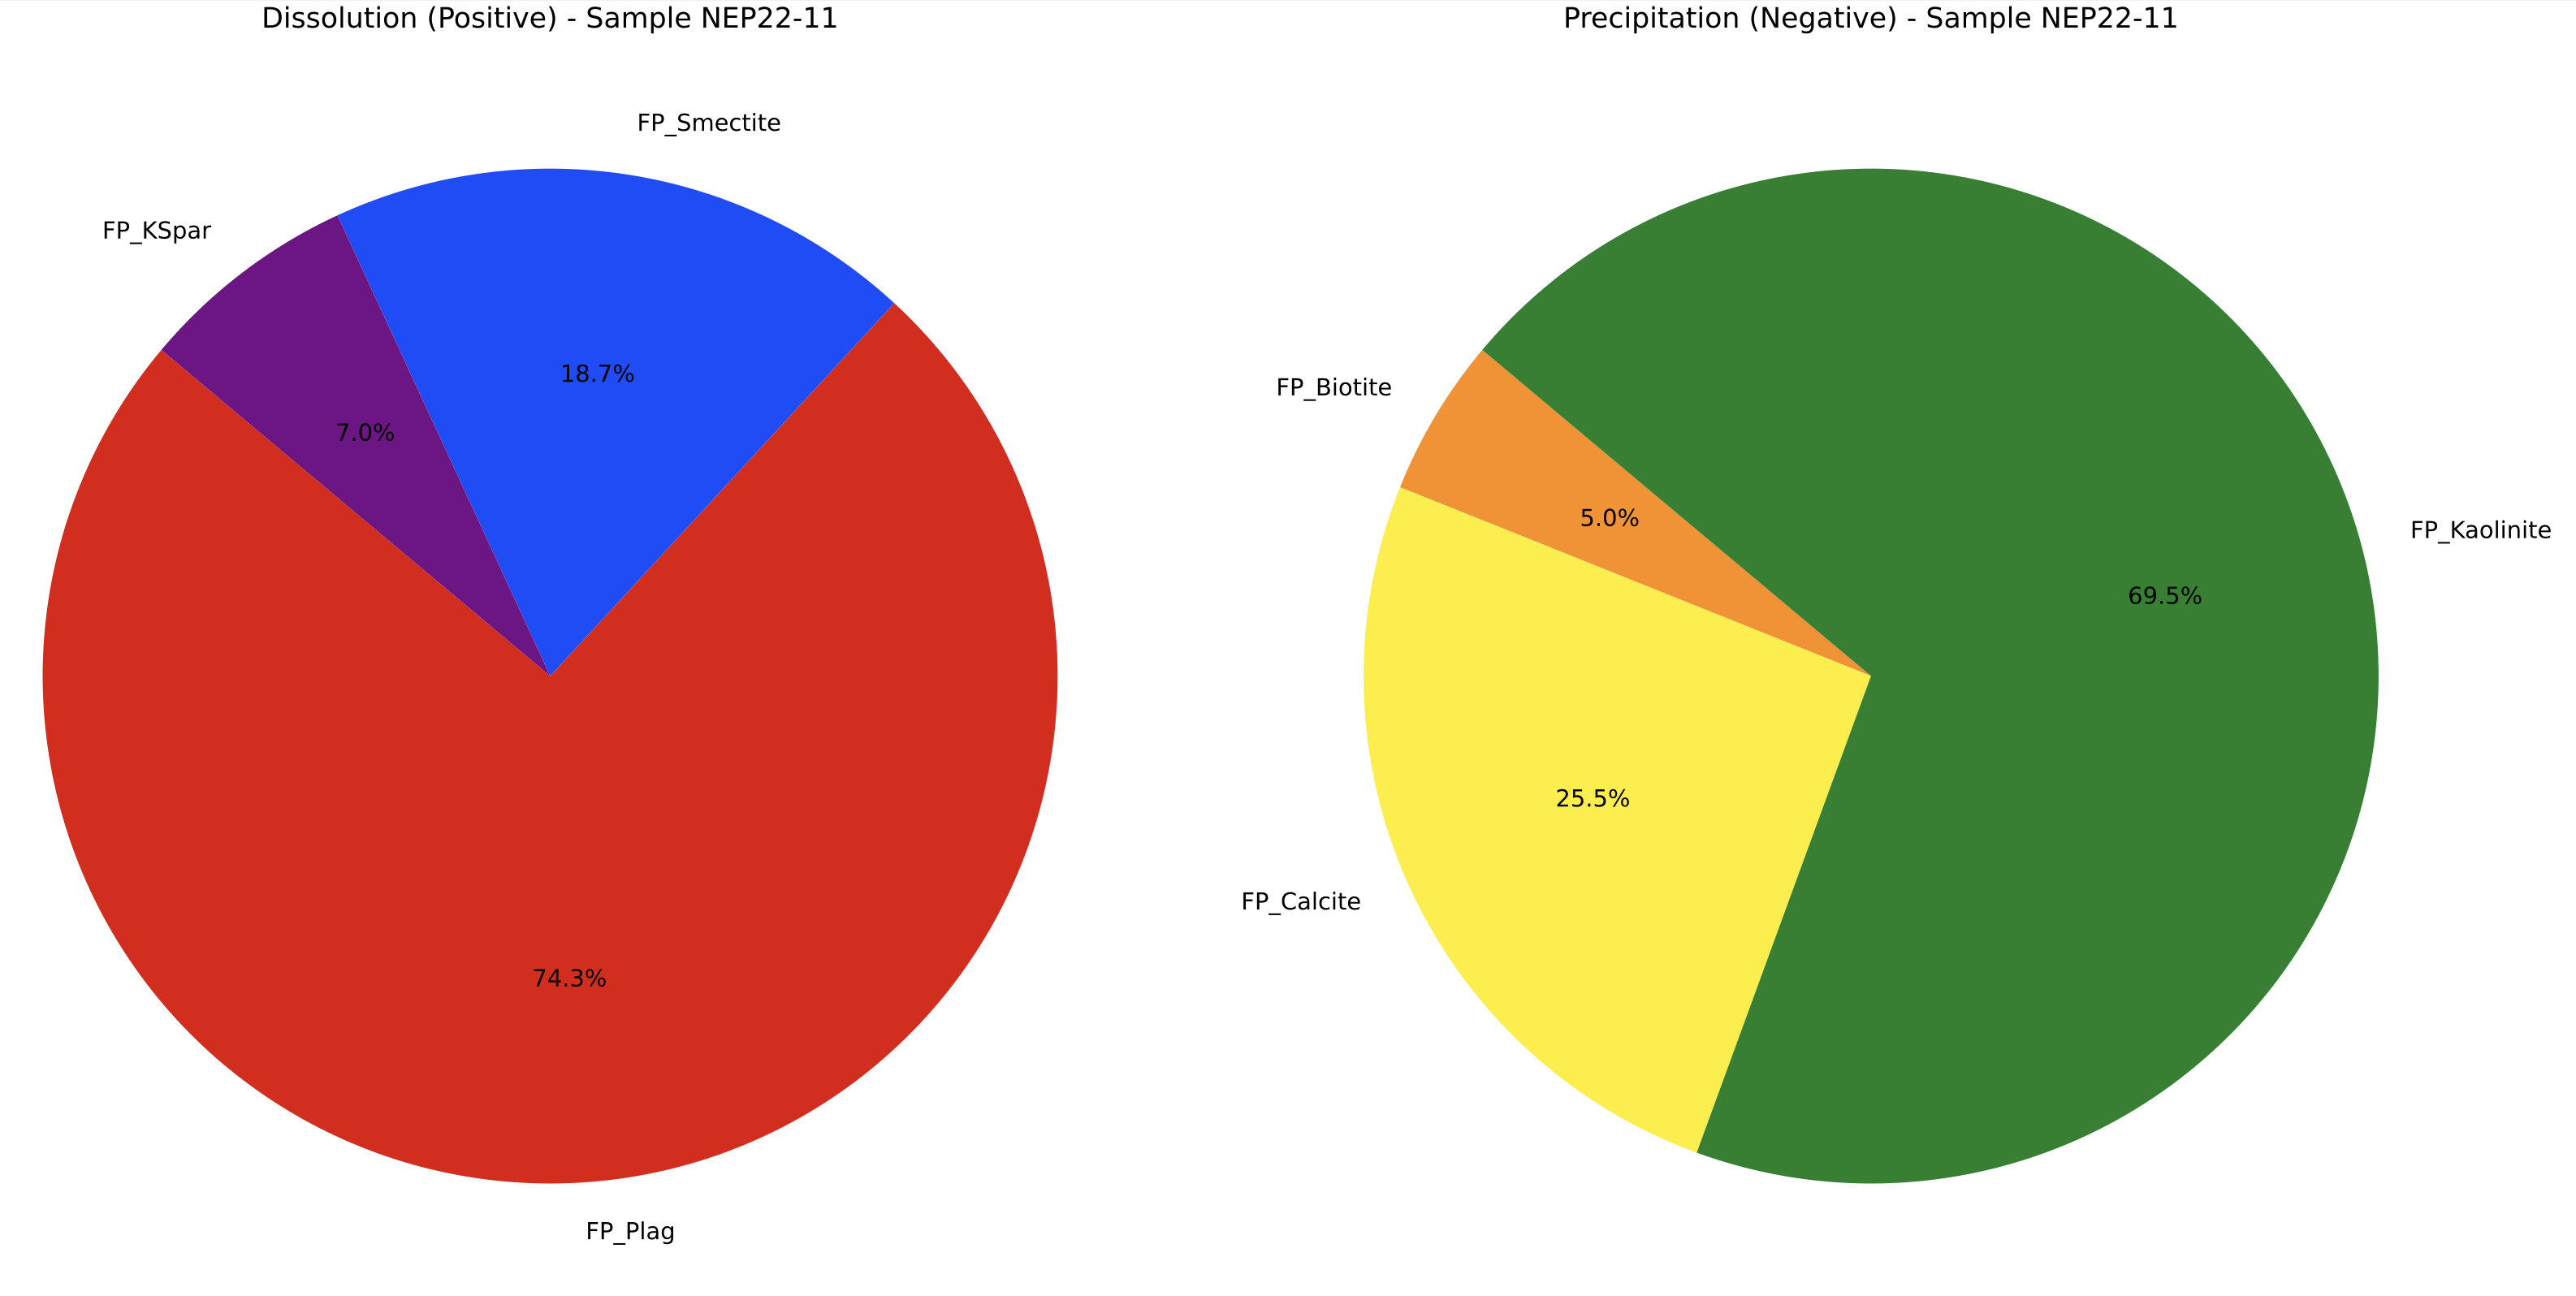
\includegraphics[width=\textwidth]{Stoichiometric_eg.png}
    \caption{Example dissolution plot}
    \label{fig:discussion6}
\end{figure}

\FloatBarrier

Figure 6 is representative of most springs in Traverse 3. Hence, the major phase being dissolved is plagioclase feldspar and the major phase being precipitated is kaolinite. The primary composition of plagioclase in the area corresponds to $\approx$ An-20 (Bickle et al., 2015; Knight et al., 2024).  The plagioclase to kaolinite reaction is given by the following equation (written so that aluminium is conserved):

\begin{equation}
    \begin{matrix}
Ca_{0.20}Na_{0.80}Al_{1.20}Si_{2.80}O_{8} + 1.2H^{+} + 0.6 H_{2}O \\ \rightarrow\\ 0.6 Al_{2}Si_{2}O_{5}(OH)_{4} + 0.8 Na^{+} + 0.2 Ca^{2+} + 1.6 SiO_{2}(aq)
    \end{matrix}
\end{equation}
\quad Or
\begin{equation}
    \begin{matrix}
An_{20} + 1.2 H^{+} + 0.6 H_{2}O\\ \rightarrow\\ 0.6 Kaolinite + 0.8 Na^{+} + 0.2 Ca^{2+} + 1.6 SiO_{2}(aq)
\end{matrix}
\label{eq:10}
\end{equation}\\



\newpage


\subsection{One-Dimensional Reactive Transport Models}

Reactive transport models are widely used in applied fluid dynamics and various fields within Earth Sciences. These models aim to track chemical reactions occurring at each spatial point, accounting for the movement of reactants to and reaction products away from those points (Bethke, 2011). The basic form of a reactive transport model is a partial differential equation that describes the transport of solutes and the reactions that occur between them. For reacting solutes, concentration changes over time are governed by transport rates—derived from the divergence principle—and the rate at which the component is introduced to or removed from the groundwater \textcolor{red}{Dissolution and Precipitation}(Bethke, 2011). The proposed equations can be complex, but in simple cases a species can be modelled to follow a first-order rate law, generally represented by\textcolor{red}{for an element concentration C\_i}:

\begin{equation}
    \frac{\partial C_i}{\partial t} = \mathcal{O}_{T}(C_i) + \mathcal{O}_{R}(C_i)
    \label{eq:1}
\end{equation}


Where \(\mathcal{O}_{T}\) and \(\mathcal{O}_{R}\) are the transport and reaction operators, respectively (Bethke, 2011). Depending on the hypothesis supported, equation \ref{eq:1} can be modified accordingly. The following sections will discuss two models with their own versions of equation \ref{eq:1}.



%Also need to make a mini 1D graphic explaining what the 1D model actually means in practice


\subsubsection{Model Motivation - \textcolor{red}{Do we add this into the other thing?}}

As discussed in the introduction, there are different hypotheses regarding the major controls on chemical weathering. This section will contrast one model following the traditional, or "null" hypothesis that weathering is largely sensitive to climate and temperature (Fontorbe et al., 2013), and another model that suggests weathering is more sensitive to fluid flux (Maher, 2011; Maher and Chamberlain, 2013). Given the emphasis on deriving fluid residence times from solute concentrations, the benchmark for a model's effectiveness will be how well it can predict these times compared to previous studies on gas tracers and simple box models. Assumptions and constraints will be compared and contrasted, and their results used to inform the calculation of rates of reaction and approach to equilibrium in Melamchi. \textcolor{red}{Why do we use Si?}



\newpage


\subsubsection{Fontorbe et al. (2013) - Null Hypothesis - Model}

This model investigates silicon isotopic composition in the Ganges River, assuming constant reaction rates along flow paths (see Appendix for a full derivation). \textcolor{red}{And see table on next part for derivation}

\bsk

The first-order differential equation governing transport and reaction is given as:\\

    \begin{equation}
    \phi \frac{\partial C}{\partial t} = -\omega \phi \frac{\partial C}{\partial z} + R_n(1-f)
    \end{equation}\\

The equation can be nondimensionalised using the Damköhler number (\(N_D\)), which describes the relative importance of kinetic vs transport-controlled settings (Bethke, 2008) \textcolor{red}{Say what everything }:\\

\begin{equation}
    N_D = \frac{R_n h}{\phi C_o \omega}
\end{equation}\\

Assuming steady-state (\(\partial C/\partial t = 0\)), the concentration at the end of the flow path can be rearranged to give the residence time \(T_f\) and reaction rate \(R_n\):\\

\begin{equation}
    T_f = \frac{(C - C_o)\phi}{(1-f)R_n}; \quad
    R_n = \frac{(C - C_o)\phi}{(1-f)T_f}
\end{equation}



\newpage

\begin{table}[h]
    \centering
    \renewcommand{\arraystretch}{1.3} % Adjust row height
    \begin{tabular}{|c|c|c|c|}
        \hline
        \multicolumn{4}{|c|}{\textbf{Fontorbe}} \\  
        \hline
        \textbf{Parameter} & \textbf{Definition} & \textbf{Units} & \textbf{Formula (Value)} \\  
        \hline
        $\phi$ & Porosity & - & - \\
        $\omega$ & Fluid velocity & m/s & - \\
        $h$ & Length of flow path & m & Variable \\
        $C$ & Concentration \@ end of flow path & $\mu$mol/L & Variable \\
        $C_0$ & Initial concentration & $\mu$mol/L & Rain Conc \\
        $f$ & Fraction reprecipitated & - & Order 0.5 \textcolor{red}{constant?}\\
        $N_D$ & Non-dimensional number & - & $N_D = \frac{R_n h}{\phi C_0 \omega}$ \\
        $T_f$ & Residence time & $10^{-9}$ s & $T_f = \frac{h}{\omega}$ \\
        $R_n$ & Reaction rate & mol/m$^3$/s & $k\cdot S \cdot \rho \cdot 1000 \cdot X $ \\
        $k$ & Reaction rate constant & mol/m$^2$/s & - \\
        $S$ & Specific surface area & m$^2$/g & - \\
        $\rho$ & Mineral density & kg/m$^3$ &  \\
        $X$ & Volume fraction of mineral in rock & $g_{min}/g_{rock}$ & 0.2 \\
        \hline
    \end{tabular}
    \caption{Key parameters and definitions for the Fontorbe model.}
    \label{tab:parameters1}
\end{table}


\FloatBarrier









\newpage




\subsubsection{Maher Model - \textcolor{red}{Correct this with respect to mike}}


This model is built to simulate hydrological processes controlling silicate weathering. The model is based on the assumption that the reaction rate decreases linearly with approach to equilibrium. The motivation behind the hydrological control is based on sensitivity analyses of real catchment data on one-dimensional reactive transport models that this study will be investigating, which suggest that porosity, mineral surface area, and temperature have no consistent correlation with water composition (Maher, 2011). The model begins with the following representation of the concentration of a solute in a fluid flow path:\\ 

\begin{equation}
\frac{dc}{dt} = -\frac{q}{\theta} \frac{dc}{dx} + \sum_{i} \mu_i R_{d,i} \left( 1 - \left( \frac{c}{c_{\text{eq}}} \right)^{n_i} \right)^{m_i} - \sum_{i} \mu_i R_{p,i} \left( 1 - \left( \frac{c}{c_{\text{eq}}} \right)^{n_i} \right)^{m_i}
\end{equation}\\

Where c is the concentration \textcolor{red}{of the element}, q is the fluid flux, theta is the volumetric water content, x is the position along the flow path, mu is the stoichiomeric coefficient, R is the rate of reaction for dissolution and precipitation respectively, c$_{eq}$ is the concentration at equilibrium, and n and m are non-linear parameters (Maher and Chamberlain, 2013). Maher and Chamberlain describe that the reaction rate decreases linearly with approach to equilibrium. \textcolor{red}{Rn is defined as:} \\

\begin{equation}
R_n = \sum_{i} \mu_i R_{d,i} - \sum_{i} \mu_i R_{p,i}
\end{equation} 
\begin{equation}
\frac{dc}{dt} = R_n \left( 1 - \frac{c}{c_{\text{eq}}} \right)
\end{equation} \\

This can be solved for \( c \), and rearranged for residence time and the rate of reaction to obtain (following Maher and Chamberlain, 2013):\\
\textcolor{red}{And note the e\^2 term because it simulates to equilibrium eg}

\begin{equation}
    T_f = \frac{C_{eq} \cdot \left(C - C_0\right)}{e^2 R_n \left( C_{\text{eq}} - C \right)};  \quad
    R_n = \frac{C_{eq} \cdot \left(C - C_0\right)}{e^2 T_f \left( C_{\text{eq}} - C \right)}
\end{equation}\\


\begin{table}[h]
    \centering
    \renewcommand{\arraystretch}{1.3} % Adjust row height
    \begin{tabular}{|c|c|c|c|}
        \hline  % DOUBLE BOLD LINE
        \multicolumn{4}{|c|}{\textbf{Maher}} \\  
        \hline
        \textbf{Parameter} & \textbf{Definition} & \textbf{Units} & \textbf{Formula (Value)} \\  
        $L$ & Length of flow path & m & Variable \\
        $q$ & Flow rate & m/s & Variable \\
        $\phi$ & Porosity & - & 0.3 (but variable) \\
        $\theta$ & Volumetric water content & - & Variable \\
        $R_n$ & Net reaction rate & mol/L/s & $\rho_{sf} \cdot k \cdot A \cdot X_r $ \\
        $\rho_{sf}$ & Mass mineral / Fluid Volume ratio & g/L & $1000 \cdot \rho_b / \phi$ \\
        $\rho_b$ & Plagioclase density & g/cm$^3$ & - \\
        $k$ & Reaction rate constant & mol/m$^2$/s & - \\
        $A$ & Specific surface area & m$^2$/g & 0.1-1 \\
        $X_r$ & Mineral concentration in fresh rock & $g_{min}/g_{rock}$& Wt\% in rock \\
        $\tau$ & Scaling factor & - & $\tau = e^2$ \\
        $D_w$ & Damkohler Coefficient & m$^2$/s & $D_w = \frac{L \phi R_n}{C_{\text{eq}}}$ \\
        $T_f$ & Residence time & $10^{-6}$ s & $T_f = \frac{L \phi}{q}$ \\
        $C_{eq}$ & Equilibrium concentration & $\mu$mol/L & Max Catchment \\
        $C_0$ & Initial concentration & $\mu$mol/L & Rain Conc \\
        \hline
    \end{tabular}
    \caption{Key parameters and definitions for the Maher model.}
    \label{tab:parameters2}
\end{table}

\FloatBarrier


\newpage

\subsubsection{Comparison of the Models}

\begin{table}[h]
    \centering
    \renewcommand{\arraystretch}{2.2} % Adjust row spacing
    \begin{tabular}{cc}
        \toprule
        \textbf{Fontorbe} & \textbf{Maher} \\
        \midrule
        $\displaystyle T_f  = \frac{\left(C_h - C_o\right)\cdot\phi}{\left(1-f\right)\cdot R_n}$ & 
        $\displaystyle T_f = \frac{C_{eq} \cdot \left(C - C_0\right)}{e^2 R_n \left( C_{\text{eq}} - C \right)}$ \\ [10pt]
        $\displaystyle R_n  = \frac{\left(C_h - C_o\right)\cdot\phi}{\left(1-f\right)\cdot T_f}$ & 
        $\displaystyle R_n = \frac{C_{eq} \cdot \left(C - C_0\right)}{e^2 T_f \left( C_{\text{eq}} - C \right)}$ \\
        \bottomrule
    \end{tabular}
    \caption{Comparison of equations from Fontorbe and Maher}
    \label{tab:equations}
\end{table}


From this table comparison, it is easy to see the differences between why the two models will differ in their estimation of residence time. The difference in the models comes from the equilibrium concentration in the Maher formula. Indeed, given that the concentration is taken from the highest in the catchment (so as not to follow Maher and Chamberlain (2013)'s rather conservative estiamte following Gaillardet et al. (1999)'s global river data)\textcolor{red}{rewrite in a nicer fashion}, the fraction

\[
\frac{C_{eq}}{C_{eq} - C}
\]\\

gets larger as the reaction progresses. As the reaction progresses, the Maher model will predict longer times than the Fontorbe model.\textcolor{red}{More about the model differences}\\ 


\begin{figure}[h]
    \centering
    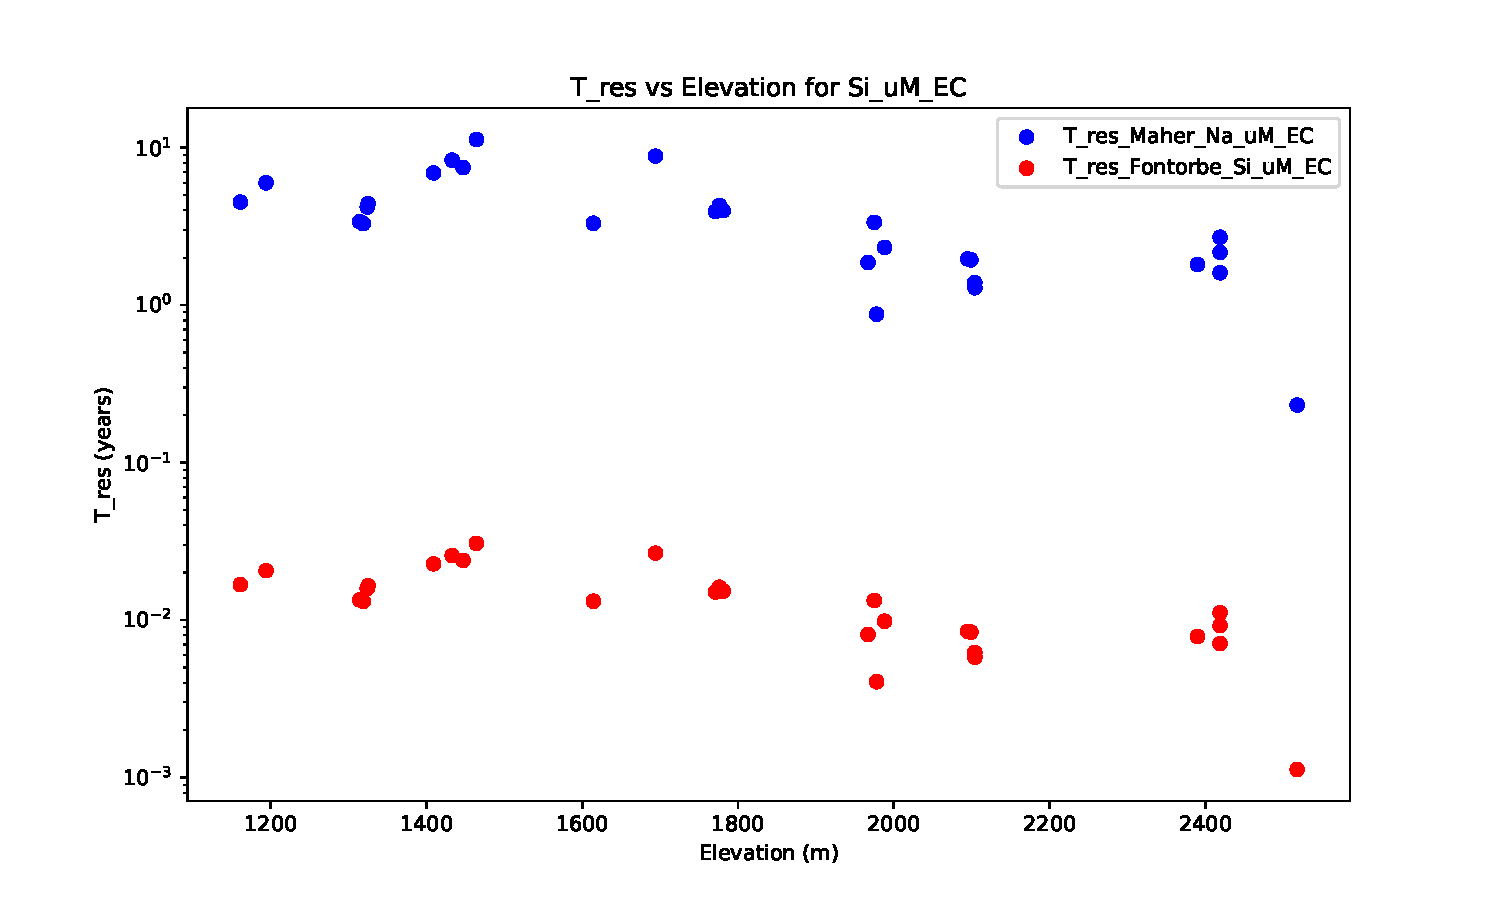
\includegraphics[width=\textwidth]{T_res_Si_uM_EC_comparison.pdf}
    \caption{Comparison for the residence time between the two models. Evaluated for Specific surface area = 0.1; Mineral concentration in rock = 0.2; density of plagioclase = 2700; Reaction rate constant = 10e-15; Porosity = 0.1; Equilibrium concentration = Max in the catchment = 800 uM; Initial concentration = smallest in the traverse; Fraction reprecipitated = 0.5.}
    \label{fig:discussion7}
\end{figure}

\FloatBarrier


As expected, the Fontorbe model predicts older times at short flow paths, and the Maher model predicts older times at longer flow paths. This difference is due to the formulation of the rate of reaction, which is constant in the Fontorbe model but depends on the equilibrium concentration for the Maher model. Indeed, as equilibrium concentration is reached, the reaction rate will decrease, and the residence time will increase. It is unrealistic that reaction rate continue to be constant as the reaction progresses, and so the Maher model is more appropriate to describe catchment-wide settings such as this. This is illustrated in the following graphic: \textcolor{red}{But DO they approach equilibrium?? See next section eg}

\begin{figure}[h]
    \centering
    \includegraphics[width=0.8\textwidth]{TheoreticalCeq.pdf}
    \caption{Comparison of how concentration changes with flow path length for the two models, and different equilibrium concentration}
    \label{fig:discussion8}
\end{figure}

\FloatBarrier



\newpage


\subsubsection{Constraints on Residence Time}

As per Acharya et al. (2020), parts of the literature suggest that the most amount of precipitation occur in the top quarter of the Himalayan catchments. \textcolor{red}{see lit review eg}Studies analysing gas ages %(what are they?)
suggest that the residence time of the water in this catchment is on the order of 10 years, with an average of 25 years (Atwood et al, 2020). 

\bsk

Assuming an average rainfall rate of 3.5 m/yr (cite) over the top quarter of the catchment which is approximately 1km long, a m2/yr rate of 3500 is obtained. When considering a 10m wide channel flow of water, a flow rate of 350 m/yr for the top quarter of the catchment is obtained. \textcolor{red}{Need more meat on this..}

\bsk

Secondly, using the oxygen isotopic composition of the springs, and comparing to the rainfall line, it is possible to obtain a flow path length assuming a general slope of 20 degrees:



\begin{figure}[h]
    \centering
    \includegraphics[width=\textwidth]{IMG_1913.pdf}
    \caption{Proving the point that residence time is around 10 years}
    \label{fig:discussion7}
\end{figure}

\FloatBarrier

% \begin{figure}[h]
%     \centering
%     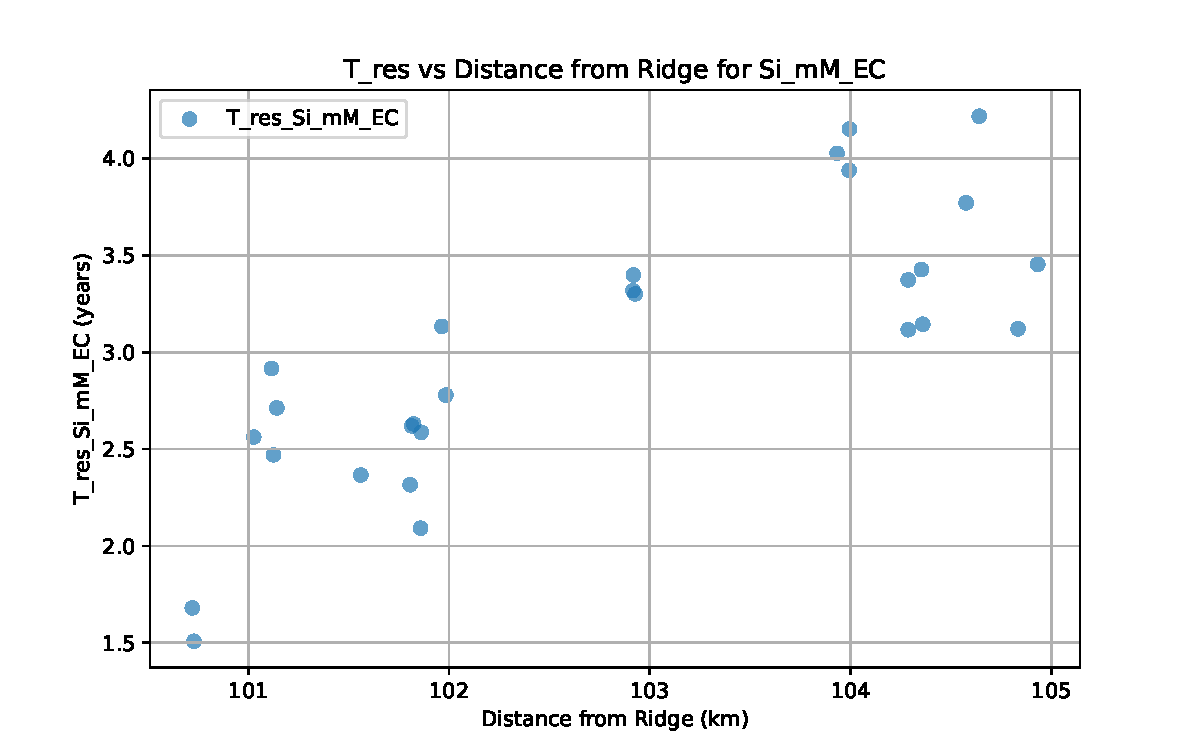
\includegraphics[width=\textwidth]{T_res_DistanceSi_mM_EC.pdf}
%     \caption{Residence time against distance from the ridge crest for the Maher model. Should we do elevation instead?}
%     \label{fig:discussion7}
% \end{figure}

% \FloatBarrier


In this way it is plausible that ~10 years could be how long the water is spending in the catchment, consistent with the \textcolor{red}{both} models. Such a finding suggests that the delay in river discharge of Andermann et al. (2013) is likely only recording surface or near-surface flow. The shorter flow paths here could plausibly be associated to residence times of a few months. 

\newpage



\subsection{Free Energy Calculations}

A further constraint on the approach to equilibrium of a water packet is the free energy of reaction, which can be calculated using the activity of the ions in solution. Free energy is defined as:\textcolor{red}{cite}

\begin{equation}
    \Delta G = \Delta G^0 + RT \ln Q
\end{equation}

The plagioclase to kaolinite reaction is given by equation \ref{eq:10}. The parameters for the standard free energy of reaction are calculated using the pygcc python package (cite). The package gives the standard properties of solid-solution species and reactions, such that $\Delta G^0$ can be calculated:

\begin{equation}
    \Delta G^0 = \Delta G^0_{products} - \Delta G^0_{reactants} = -RT \ln K
\end{equation}\\
K is calculated using the database obtained from pygcc using The Geochemist's Workbench® Rxn program. Q is calculated as the ion activity product of the reaction, assuming an ideal system whereby the activity is equal to the concentration of the ion in the water \textcolor{red}{Assuming the activities of the solid phases plagioclase and kaolinite are 1, the activity of water is 1, and the activity of the ions in solution are equal to their concentration, the free energy of reaction can be calculated. }

\begin{equation}
    Q = \frac{a_{\mathrm{Kaol}}^{0.6}\,a_{\mathrm{Na}^{+}}^{0.8}\,a_{\mathrm{Ca}^{2+}}^{0.2}\,a_{\mathrm{SiO_{2}(aq)}}^{1.6}}
           {a_{\mathrm{An_{20}}}\,a_{\mathrm{H}^{+}}^{1.2}}
\end{equation}\\

It is important to note that the composition of the plagioclase is important. The free energy of reaction is lowered by the presence of a solid solution between albite and anorthite (Dubacq, 2022). \textcolor{red}{In our case...}

\newpage

\subsubsection{Comparison with Residence Time}

\textcolor{red}{Need to write }
\begin{figure}[H]
    \centering
    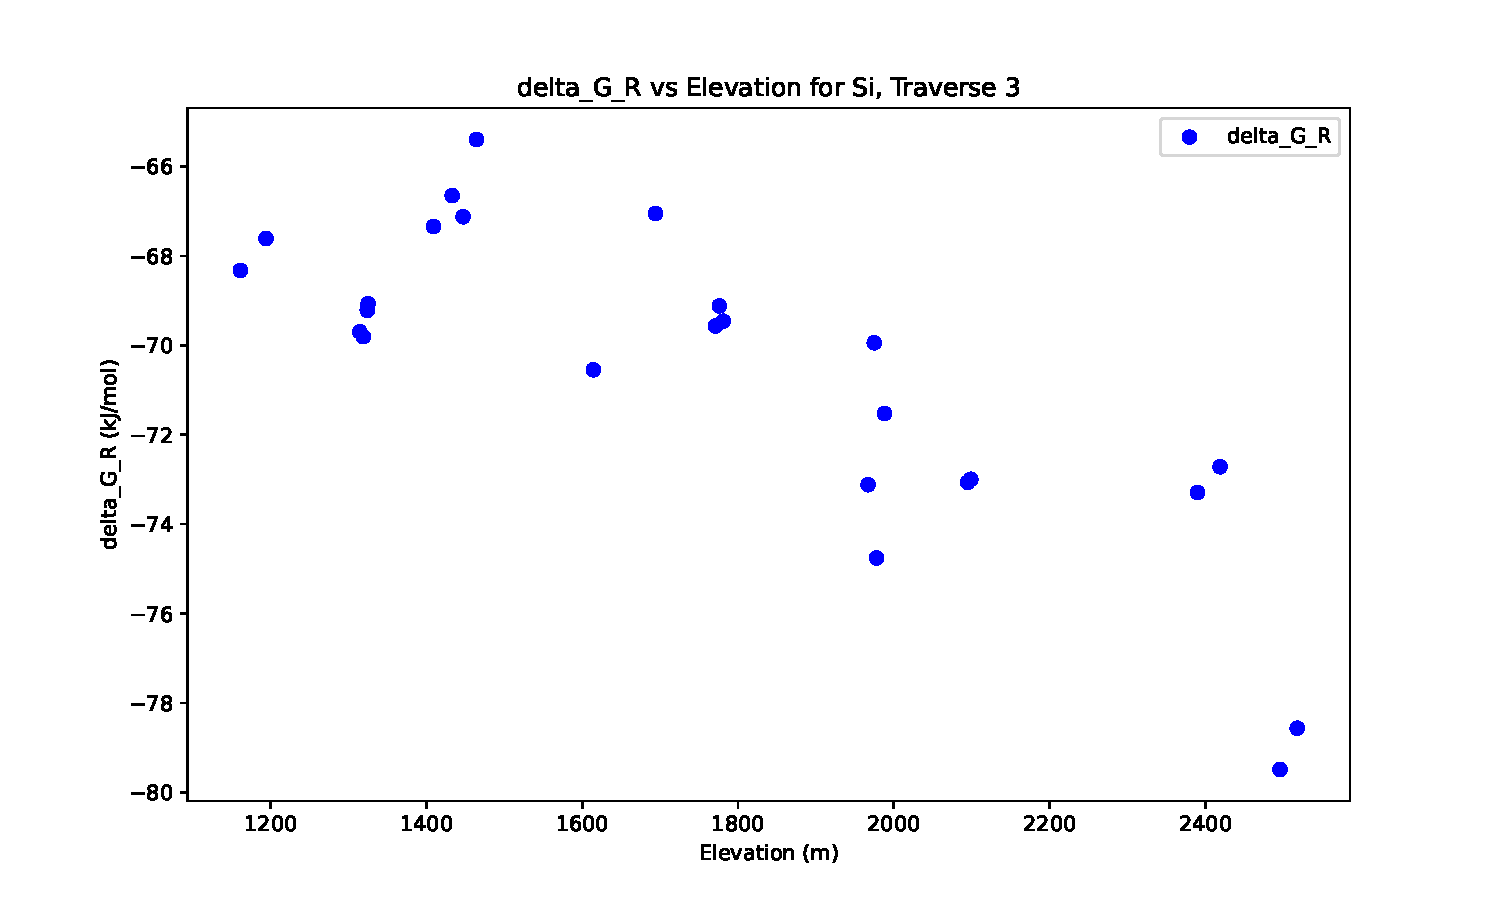
\includegraphics[width=0.9\textwidth]{delta_G_R_Si_comparison.pdf}
    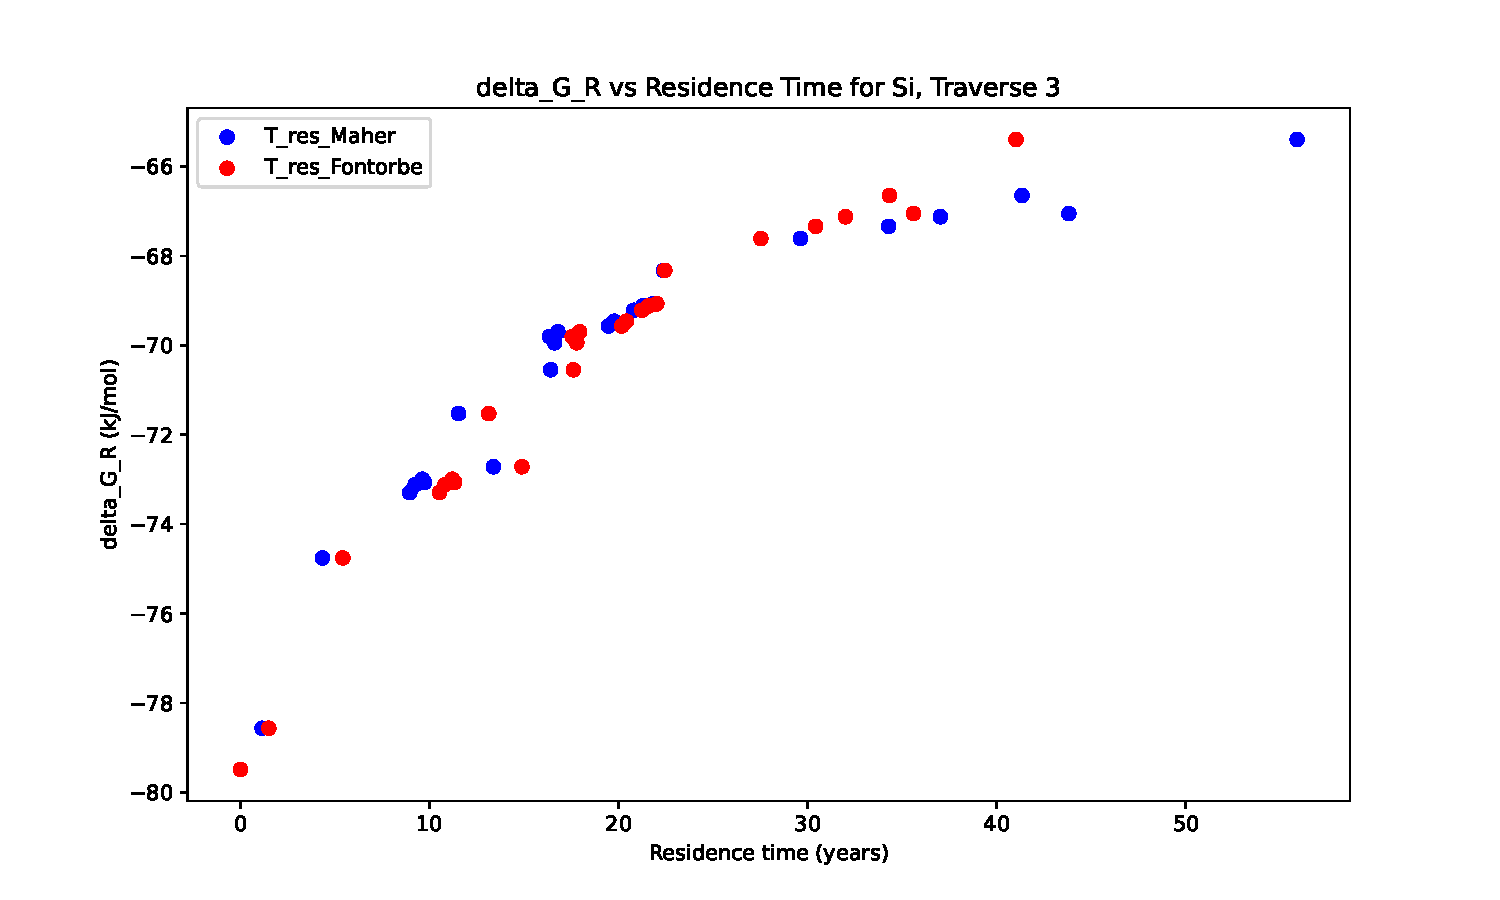
\includegraphics[width=0.9\textwidth]{delta_G_R_Si_time.pdf}
    \caption{Comparison of the delta G obtained against elevation. Comparison of delta G with residence time for both models}
    \label{fig:discussion8}
\end{figure}

\FloatBarrier


\newpage

\subsubsection{Constraints on Reaction Rate}

Figure \ref{fig:discussion8} shows a convincing trend of decrease in $\Delta G$ as elevation decreases, consistent with the water samples getting closer to equilibrium as they flow for more time, and so the reaction occurs more. However, the free energy is only on the order of -60 kJ/mol at the longest flow path. This is not close to the -10kJ/mol that Kampman et al. (2014) suggest is the "near equilibrium plateau". There might be an argument, therefore, to suggest that the reaction rate is not as high as the models suggest. Indeed, at those values, laboratory rates might be more appropriate \textcolor{red}{Have the Kampman table? Lab rates of reaction are much faster for this }. One sure test is to compare the free energy obtained for the samples in Traverse 3 to those in Traverse 1. Given that the equilibrium concentration for the residence time is taken from this latter traverse (see Figure in results, ref), according to the formulation of the Maher model this should be closest to equilibrium.

\bsk

Figure \ref{fig:discussion9} does indeed show that the free energy of reaction is lower for the samples in Traverse 1 than in Traverse 3. However, the maximum value reached is still far away from equilibrium. Hence, it is likely that a larger reaction rate is needed to characterise these groundwaters. This has implications for the residence times calculated using these models, as the former and latter are inversely proportional.


\textcolor{red}{Bit about Maher assuming equilibrium reached -> Maher not correct to implement here. Also mike permeability sketch???}


\begin{figure}[h]
    \centering
    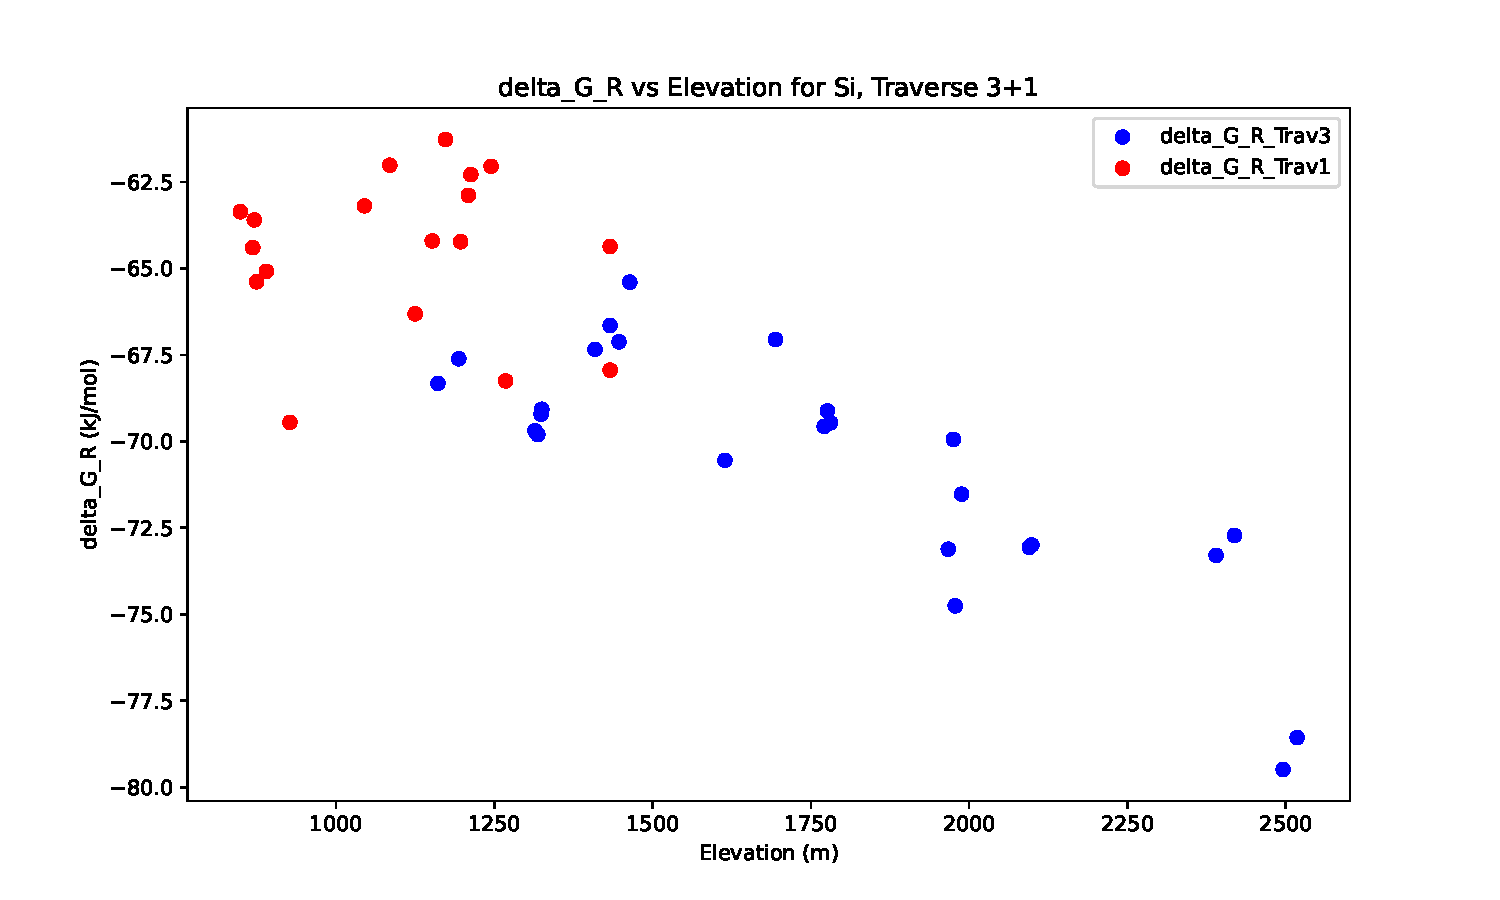
\includegraphics[width=\textwidth]{delta_G_R_Si_comparison_Trav1.pdf}
    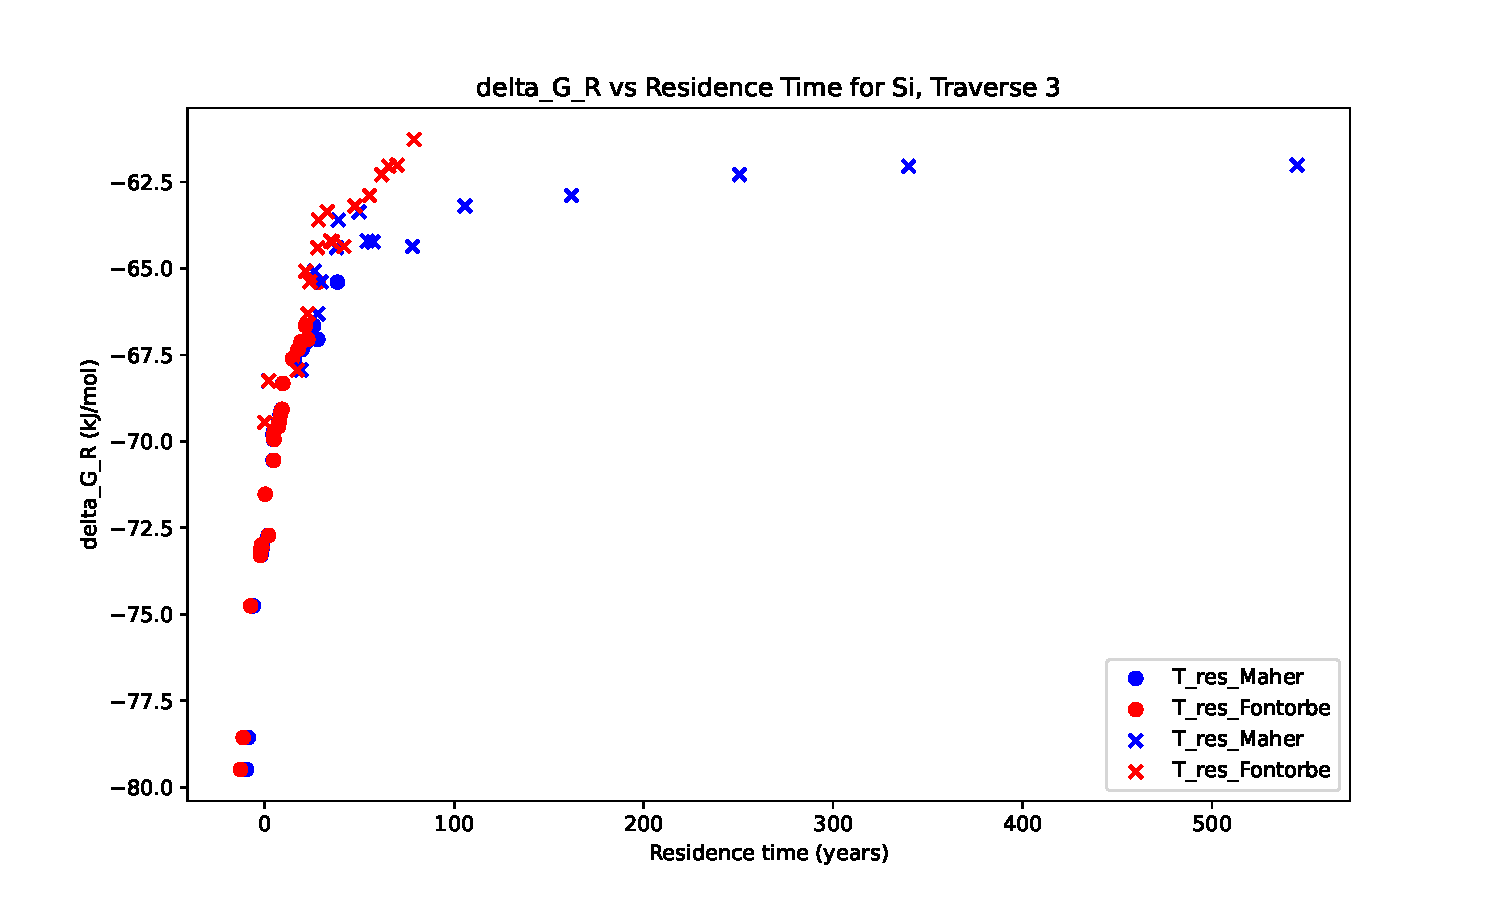
\includegraphics[width=\textwidth]{delta_G_R_Si_time_trav1.pdf}
    \caption{Comparison of the delta G obtained against elevation for Traverse 1 and Traverse 3. And residence time comparison, Note how Maher predicts really high residence times when Ceq is approached}
    \label{fig:discussion9}
\end{figure}

\FloatBarrier







\FloatBarrier


